\documentclass[11pt]{article}

\usepackage{graphicx}

\oddsidemargin=.25in
\evensidemargin=.25in
\textwidth=6in
\topmargin=0in

\parindent=0in

\begin{document}

\centerline {\Large \bf Kobby Editor Description}
\centerline {Written by Gregory Haynes}

\paragraph{}Kobby is a text editor application that allows for real time collaborative editing of documents.  Collaborative editing refers to the act of multiple users modifying one document, similar to having several people write on the same sheet of paper.  Real time refers to the ability for each user to see what is being written by all other users as they write it.

\begin{figure}[tbh]
\begin{center}
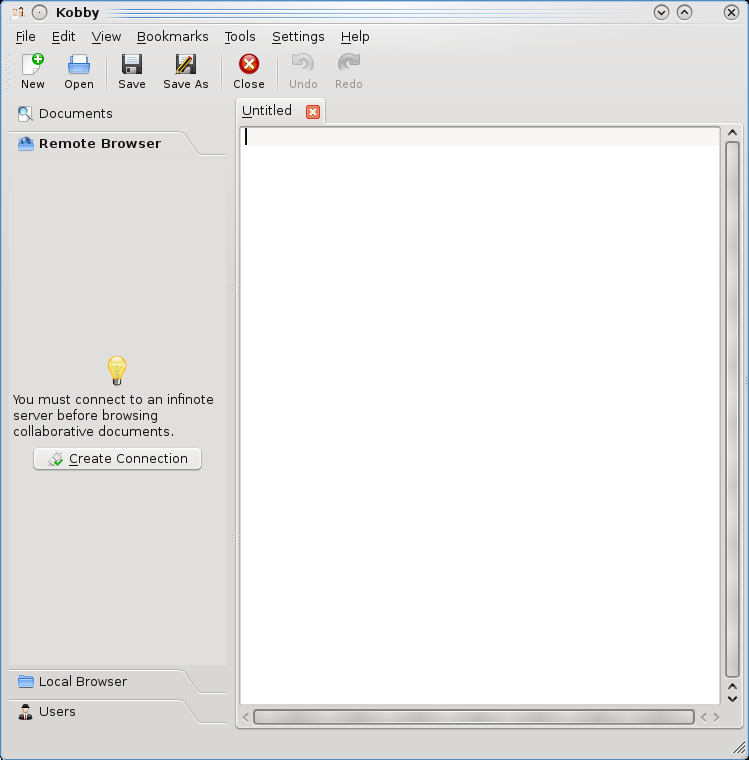
\includegraphics[width=.7\textwidth]{kobbymain.png}
\end{center}
\caption{Kobby Editor Main Window}
\end{figure}

\paragraph{}The Kobby application consists mainly of a text editor window.  This window contains a central text editing area where the editing of documents is performed.  There are also two panels in this window, a actions panel on the top edge of the window and a toolbox panel on the left edge.  The actions panel features quick-access buttons similar to those found on most other text editors.  These buttons allow the user to create new documents, open existing documents, and save or close a document being edited.  The toolbox displays information about currently opened documents, and contains a browser for joining collaboratively edited documents.

\paragraph{}In addition to the main editor window, the Kobby application features several dialogs which allow the user to supply information.  A dialog refers to any window which opens seperate from the main window, such as the file browser dialog used when opening documents.  One dialog in the Kobby application is a welcome dialog, which contains text entry boxes for a username and hostname.  Kobby also contains a file browser dialog which contains a selectable browser window of files on the computer, and a create connection dialog containing three text input boxes for a name, hostname, and port.

\end{document}